% Modeling
This chapter begins with the models and derivations for the case of one dimensional time reversal and is based upon work performed by Korde \cite{Fehrman2012}. Following that material will be a brief overview of two dimensional time reversal which is drawn from a number of published sources.

\section{One Dimensional Wave Equation}
\label{sec:oneDWaveEquation}

In this section the one dimensional wave equation for a linear elastic material with uniform density and cross-sectional area will be derived. The derivation is based on knowledge from numerous books such as Kolsky \cite{Kolsky1963} and Brown et. al. \cite{Brown2008}.

\begin{figure}[ht!]
\centering
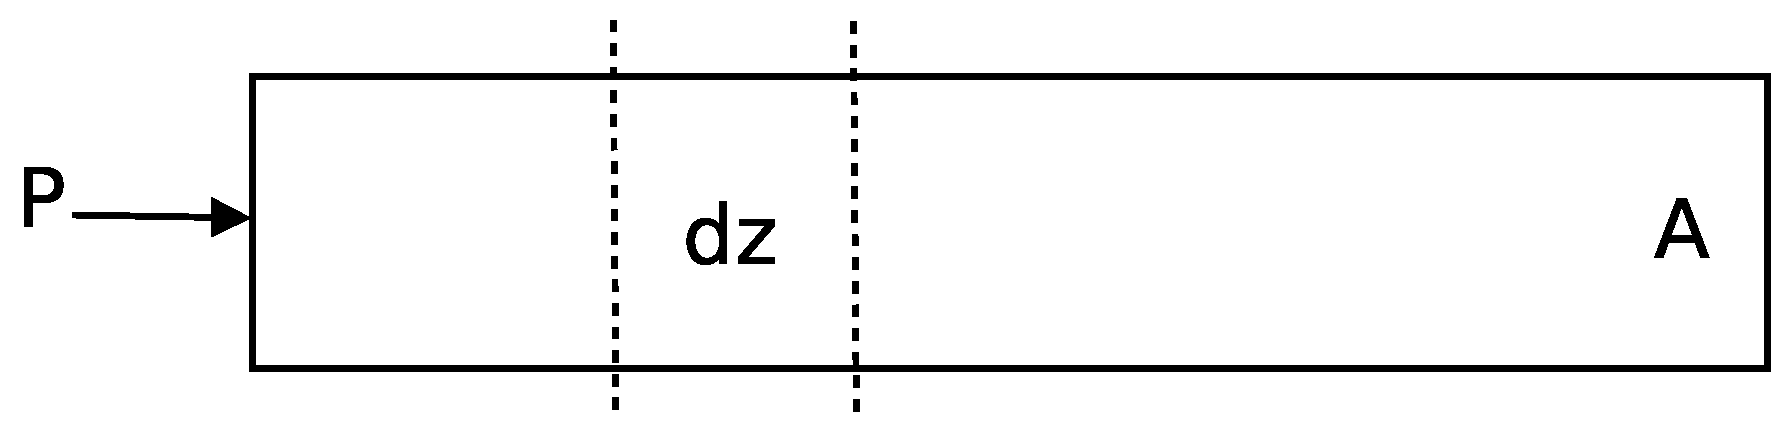
\includegraphics[width=0.8\textwidth]{eps_pics/deriveWaveRod}
\caption{Diagram for deriving the one dimensional wave equation given an axial pressure applied to one end of the material with uniform density and cross-sectional area.
	 \label{fig:deriveWaveRod}} 
\end{figure}

Figure \ref{fig:deriveWaveRod} gives a basic diagram that is used for the wave equation derivation, with $P$ being the axial pressure, $dz$ being the material's differential element of length, and $A$ being the cross-sectional area of the material. Define the stress in the z direction as:

\begin{equation}
T_3 = \frac{P}{A}
\end{equation}

\nomenclature{$P$}{Axial pressure applied to rod end}
\nomenclature{$A$}{Cross-sectional area of the rod}
\nomenclature{$dz$}{Differential element of length for the rod}
\nomenclature{$T_3$}{Stress in the z direction}

\begin{figure}[ht!]
\centering
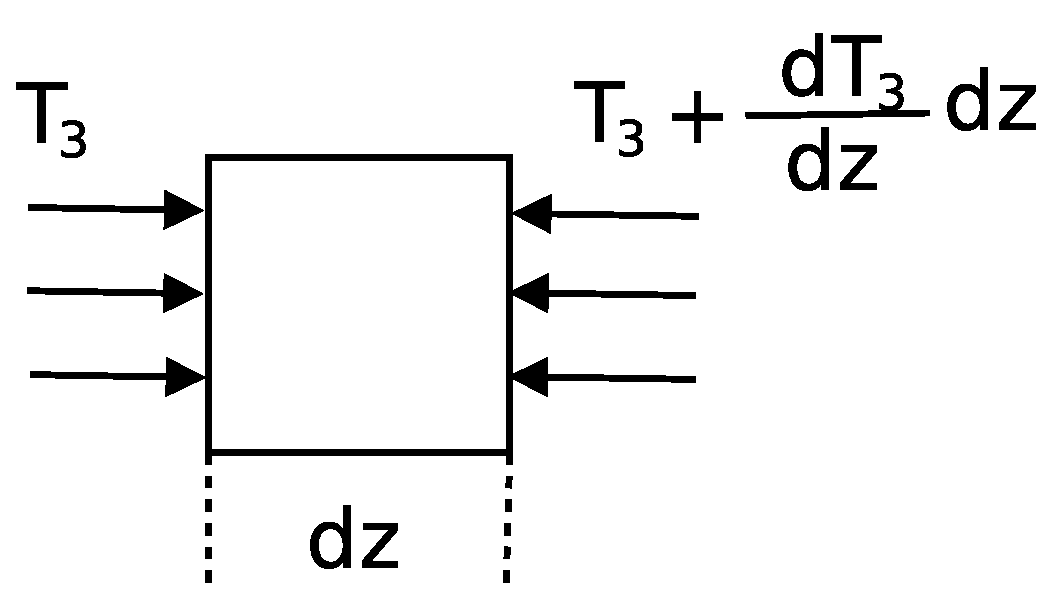
\includegraphics[width=0.8\textwidth]{eps_pics/diffElementRod}
\caption{Differential element showing the stresses acting on the rod.
	 \label{fig:diffElementRod}} 
\end{figure}

Applying Newton's second law and summing the forces,

\begin{equation}
-T_3A + (T_3 + \frac{dT_3}{dz}dz)A = A\rho^* dz \frac{d^2w}{dt^2}
\end{equation}

\nomenclature{$\rho^*$}{Density of the rod material}
\nomenclature{$w$}{Displacement of the rod}

With $\rho^*$ being the density of the rod material and $w$ being the displacement. Dividing through by the area,

\begin{equation}
-T_3 + T_3 + \frac{dT_3}{dz}dz = \rho^* dz \frac{d^2w}{dt^2}
\end{equation}

\begin{equation}
\frac{dT_3}{dz}dz = \rho^* dz \frac{d^2w}{dt^2}
\end{equation}

Canceling the $dz$ term,

\begin{equation}
\frac{dT_3}{dz} = \rho^* \frac{d^2w}{dt^2}
\label{eq:strainWave}
\end{equation}

$C^*_{33}$ is the elastic constant in the z direction and is defined as the ratio of the stress and strain in the z direction. This is given by,

\begin{equation}
C^*_{33} = \frac{T_3}{S_{33}} \implies T_3 = C^*_{33}S_{33}
\label{eq:T_3}
\end{equation}

\nomenclature{$C^*_{33}$}{Elastic constant in the z direction}
\nomenclature{$S_{33}$}{Strain in the z direction}

With $S_{33}$ being the strain in the z direction. Strain is the ratio of the change in material length to the original length and in this case is given by,

\begin{equation}
S_{33} = \frac{dw}{dz}
\label{eq:S_33}
\end{equation}

Inserting \ref{eq:S_33} in to \ref{eq:T_3} we see that

\begin{equation}
T_3 = C^*_{33}\frac{dw}{dz}
\label{eq:T_3fin}
\end{equation}

Putting \ref{eq:T_3fin} back in to \ref{eq:strainWave} and realizing that $w$ is a function of both $t$ and $z$,

\begin{equation}
C^*_{33}\frac{\partial ^2w}{\partial z^2} = \rho^* \frac{\partial ^2w}{\partial t^2}
\end{equation}

Dividing through by $\rho^*$ and moving the LHS term to the RHS, we arrive at

\begin{equation}
\frac{\partial ^2w}{\partial t^2} - c^{*2} \frac{\partial ^2w}{\partial z^2} = 0
\label{eq:waveEquationFin}
\end{equation}

\nomenclature{$c^*$}{Velocity of wave propagation through the rod}

With $c^*$ being the velocity of the wave propagation and is defined as,

\begin{equation}
c^* = \sqrt{\frac{C^*_{33}}{\rho^*}}
\end{equation}

\section{Piezoelectric transducers}

This section describes the governing equations for $d_{33}$ piezoelectric transducers that are placed on each end of a rod. The following work is based on derivations by Dr. Korde.

The constitutive equations for the transducers are:

\begin{equation}
T_3 = \overline{C_{33}} S_3 + \overline{d_{33}} D_3
\end{equation}

and 

\begin{equation}
D_3 = \overline{\epsilon ^T_{33}} E_3 + \frac{d_{33}}{s^E_{33}} S_3
\end{equation}

\nomenclature{$D_3$}{Electric displacement in the z direction}
\nomenclature{$E_3$}{Electric field intensity in the z direction}
\nomenclature{$d_{33}$}{Strain constant relating the strain and field intensity in the z direction}

Where $D_3$, $E_3$, and $d_{33}$ are the electric displacement, electric field intensity, and the strain constant relating strain and field intensity, respectively, all in the z direction. The other variables are given by the following equations:

\begin{equation}
s^E_{33} = \frac{1}{C_{33}}
\end{equation}

\begin{equation}
\overline{C_{33}} = \frac{1}{s^E_{33}(1 - \frac{d^2_{33}}{s^E_{33}\epsilon ^T_{33}})}
\end{equation}

\begin{equation}
\overline{d_{33}} = -\frac{d_{33} / \epsilon ^T_{33}}{s^E_{33}(1 - \frac{d^2_{33}}{s^E_{33}\epsilon ^T_{33}})}
\end{equation}

\begin{equation}
\overline{\epsilon ^T_{33}} = -\frac{\epsilon ^T_{33}}{s^E_{33}(1 - \frac{d^2_{33}}{s^E_{33}\epsilon ^T_{33}})}
\end{equation}

\nomenclature{$C_{33}$}{PZT elastic constant in the z direction}
\nomenclature{$\epsilon ^T_{33}$}{PZT permittivity constant for the z direction}

With $C_{33}$ and $\epsilon ^T_{33}$ being the PZT elastic constant in the z direction and permittivity constant in the z direction respectively.

\begin{figure}[ht!]
\centering
\includegraphics[width=1\textwidth]{eps_pics/trans_circ}
\caption{Equivalent circuit diagram for the piezoelectric transducers.
	 \label{fig:trans_circ}} 
\end{figure}

\nomenclature{$C_c$}{Equivalent capacitance for the transducers}

The equivalent circuits for the transducers are modeled as a resistor and capacitor in series as shown in Figure \ref{fig:trans_circ} and with $C_c$ being the equivalent capacitance and is given by

\begin{equation}
C_c = \overline{\epsilon_{33}} \pi a^2/l
\end{equation}

\nomenclature{$a$}{Transducer cross sectional area}
\nomenclature{$l$}{Transducer length}
Where $a$ and $l$ are the transducer area and length respectively. 

\section{Rod with Transducers}
\label{sec:rodWithTrans}

\begin{figure}[ht!]
\centering
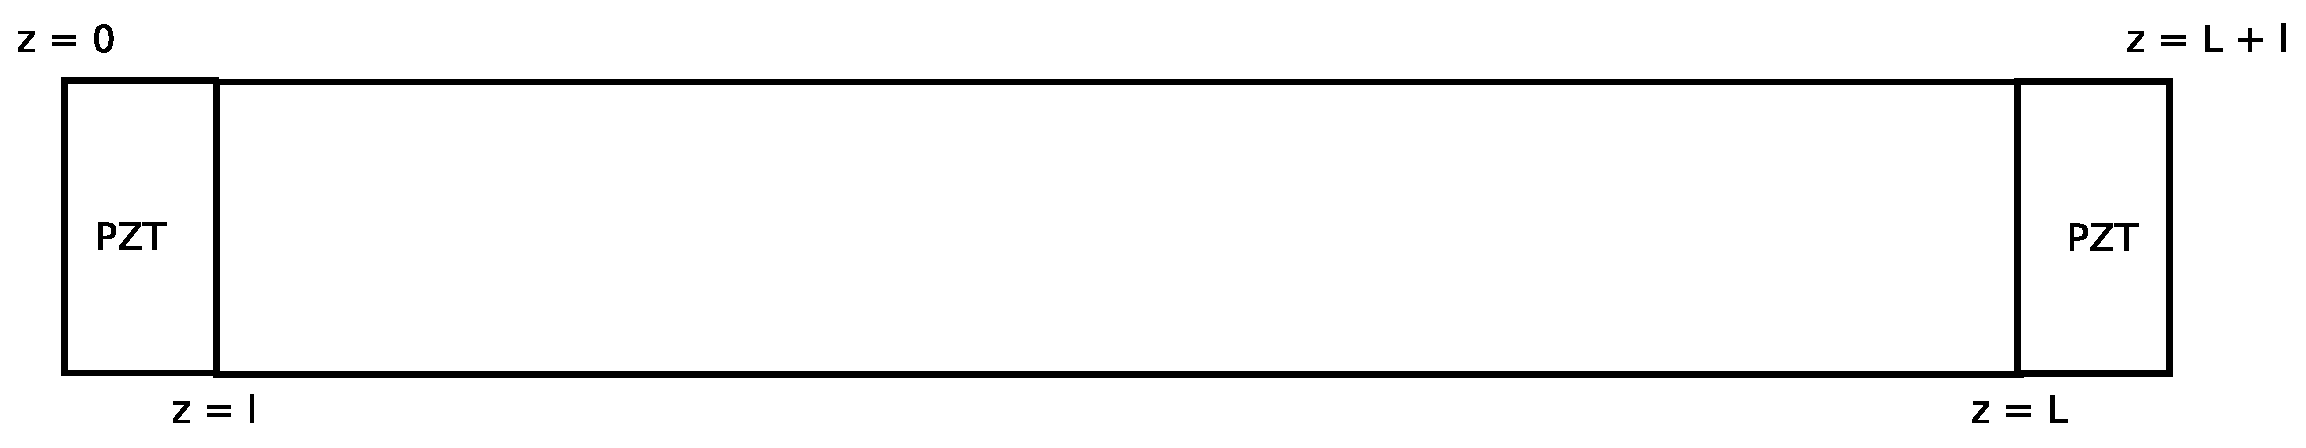
\includegraphics[width=0.8\textwidth]{eps_pics/rodTrans.eps}
\caption{Diagram of a rod with $d_{33}$ piezoelectric transducers placed on each end.
	 \label{fig:rodTrans}} 
\end{figure}

Consider a rod with $d_{33}$ transducers affixed to each end as pictured in Figure \ref{fig:rodTrans}. We wish to model propagation of a wave through the system with the wave being sent by one of the transducers. The one-dimensional wave results from Section \ref{sec:oneDWaveEquation} can be applied here such that the equation of the motion for the wave propagating through the transducers is the same as through the rod but with a different density and elastic coefficient which will be denoted as $\rho$ and $C_{33}$ respectively. The wave velocity through the transducer is then described as

\begin{equation}
c = \sqrt{\frac{C_{33}}{\rho}}
\end{equation}

\nomenclature{$\rho$}{Density of the transducer material}

So for $0 \le z \le l$ and $L < z \le (L+l)$ we have

\begin{equation}
\frac{\partial ^2w}{\partial t^2} - c^2 \frac{\partial ^2w}{\partial z^2} = 0
\label{eq:transWaveEquationFin}
\end{equation}

For the rod domain, $l < z \le L$, we just apply equation \ref{eq:waveEquationFin}. Let the stress and deflection across the interfaces be continuous. When a wave encounters either of the interfaces it will experience refraction in which part of the wave will be reflected and part will be transmitted into the next medium. This phenomena can be accounted for by finding the reflection and transmission coefficients for each interface. For $z = l$ these coefficients are found to be

\begin{equation}
\boldsymbol{R} = \frac{\overline{C_{33}} + \frac{\overline{d_{33}}d_{33}}{2s^E_{33}} - C^*_{33}}{\overline{C_{33}} + \frac{\overline{d_{33}}d_{33}}{2s^E_{33}} + C^*_{33}}
\end{equation}

\begin{equation}
\boldsymbol{T} = \frac{2(\overline{C_{33}} + \frac{\overline{d_{33}}d_{33}}{2s^E_{33}})}{\overline{C_{33}} + \frac{\overline{d_{33}}d_{33}}{2s^E_{33}} + C^*_{33}}
\end{equation}

\nomenclature{$\boldsymbol{R}$}{Reflection coefficient at $z = l$}
\nomenclature{$\boldsymbol{T}$}{Transmission coefficient at $z = l$}

Similarly, for the interface at $z = (L + l)$

\begin{equation}
\boldsymbol{\hat{R}} = \frac{\overline{C_{33}} - \frac{\overline{d_{33}}d_{33}}{2s^E_{33}} - C^*_{33}}{\overline{C_{33}} + \frac{\overline{d_{33}}d_{33}}{2s^E_{33}} + C^*_{33}}
\end{equation}

\begin{equation}
\boldsymbol{\hat{T}} = \frac{2C^*_{33}}{\overline{C_{33}} + \frac{\overline{d_{33}}d_{33}}{2s^E_{33}} + C^*_{33}}
\end{equation}

\nomenclature{$\boldsymbol{\hat{R}}$}{Reflection coefficient at $z = (L+ l)$}
\nomenclature{$\boldsymbol{\hat{T}}$}{Transmission coefficient at $z = (L = l)$}

\section{Cracked Rod with Transducers}
\label{sec:rodTransCrack}

\begin{figure}[ht!]
\centering
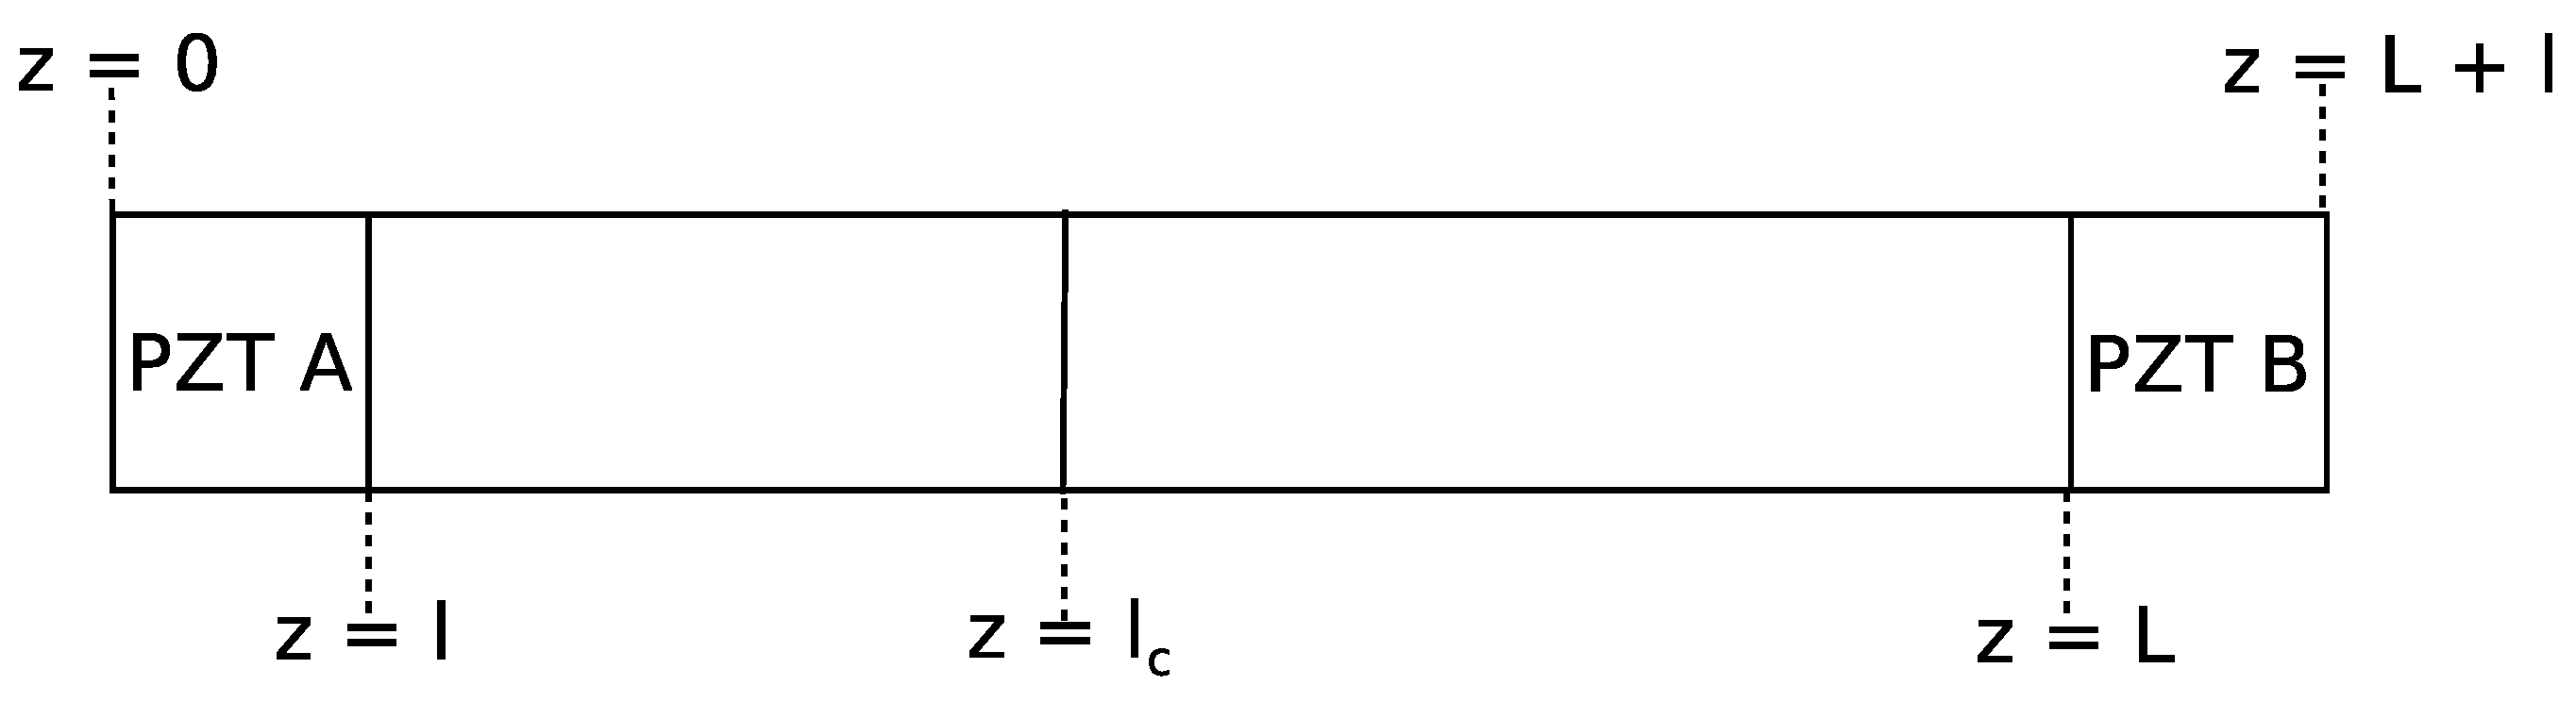
\includegraphics[width=0.8\textwidth]{eps_pics/rodTransCrack.eps}
\caption{Diagram of a rod with $d_{33}$ piezoelectric transducers placed on each end and a crack located at an arbitrary location within the system, with $l_c$ being the distance of the crack from the origin and is not known a prior.
	 \label{fig:rodTransCrack}} 
\end{figure}


In this section a crack located at an arbitrary position is introduced into the system modeled in Section \ref{sec:rodWithTrans} and is shown in Figure \ref{fig:rodTransCrack}. The crack can be modeled as another interface boundary within the system as we saw previously. If a stress wave is played out from one of these transducers, say transducer A, then it will travel through the rod and refracts upon reaching the crack location due to a change in the medium. The crack can then be accounted for as a change in the material density and elastic coefficient from $\rho ^*$ to $\rho ^c$ and from $C^*_{33}$ to $C^c_{33}$ respectively. Again, let the stress and strain at the crack interface be continuous. As seen before we will have a reflection coefficient and a transmission coefficient which are given by

 \begin{equation}
 \boldsymbol{\overline{R}} = \frac{C^*_{33} - C^c_{33}}{C^*_{33} + C^c_{33}}
 \end{equation}
 
  \begin{equation}
  \boldsymbol{\overline{T}} = \frac{2C^*_{33}}{C^*_{33} + C^c_{33}}
  \end{equation}
  
  
  \nomenclature{$\overline{R}$}{Reflection coefficient at $z = l_c$}
  \nomenclature{$\overline{T}$}{Transmission coefficient at $z = l_c$}
  \nomenclature{$\rho ^c$}{Density of the crack}
  \nomenclature{$C^c_{33}$}{Elastic coefficient of the crack in the z direction}
  
  \section{One Dimensional Time Reversal Focusing at a Crack}
  Considered here is the time reversal playback of the system modeled thus far. First there is an interrogatory phase in which transducer A plays out a stress wave which will propagate along the rod towards transducer B on the opposite end. The strain resulting from this stress wave is taken as
  
  \begin{equation}
  \frac{\partial w}{\partial z}
  \end{equation}
  
  \nomenclature{$\frac{\partial w}{\partial z}$}{The strain resulting from the stress wave that is played by transducer A during the initial phase}
  
  When the wave reaches the crack location it will refract causing part of its energy to be transmitted and part to be reflected and is described by the coefficients shown in Section \ref{sec:rodTransCrack}. The strain caused by the wave reflected portion returning to the transducer A is
  
  \begin{equation}
  \frac{\partial w_{cr}}{\partial z} = \overline{\boldsymbol{R}}\frac{\partial w_t}{\partial z}
  \label{eq:reflStrain}
  \end{equation}
  
  For the reflected portion of the wave, its strain will be
  
    \begin{equation}
    \frac{\partial w_{ct}}{\partial z} = \overline{\boldsymbol{T}}\frac{\partial w_t}{\partial z}
    \label{eq:tranStrain}
    \end{equation}
    
    In both \ref{eq:reflStrain} and \ref{eq:tranStrain}
    
    \begin{equation}
    \frac{\partial w_t}{\partial z} = \boldsymbol{T} \frac{\partial w}{\partial z}
    \end{equation}
    
    \nomenclature{$\frac{\partial w_{ct}}{\partial z}$}{Strain caused by wave portion reflecting to transducer A}
    
    \nomenclature{$\frac{\partial w_{cr}}{\partial z}$}{Strain caused by wave portion transmitting to transducer B}
    
    This will create a voltage at transducer A which is found in the frequency domain as
    
    \begin{equation}
    V^+_a(i\omega) = -\frac{d_{33} \pi a^2}{2 s^E_{33} C_c} \frac{\partial w_{cr}}{\partial z} (i\omega)
    \end{equation}
    
    and at transducer B
    
    \begin{equation}
    V^+_t(i\omega) = \frac{d_{33} \pi a^2}{2 s^E_{33} C_c} \boldsymbol{\hat{T}}\frac{\partial w_{ct}}{\partial z} (i\omega)
    \end{equation}
    
    